Tunnistautumis- ja pääsynvalvontaprotokollia tutkitaan ja kehitetään monen eri tahon toimesta. Web Services -teknologioita standardoinut OASIS (Organization for the Advancement of Structured Information Standards) on kehittänyt XML-pohjaista SAML-kieltä tunnistautumisprotokollaksi \cite{saml_spec}. SAML tarjoaa tunnistautumisprotokollan lisäksi joukon muita web-sovellukseen liittyviä turvallisuusstandardeja \cite{next_saml}.

Myös Microsoft on kehittänyt oman Windows Live ID -standardin, joka tarjoaa tunnistautumisprotokollan \cite{open_identity}. Windows Live ID on osittain suljettu standardi, joka tarjoaa tunnistautumisprotokollan lisäksi täydellisen keskitetyn käyttäjän identiteetin hallinnan \cite{open_identity}. Suljetun lähdekoodin vuoksi Windows Live ID ei ole tämän tutkielman kannalta kiinnostava protokolla.

Avoimen lähdekoodin yhteisössä on syntynyt OpenID, jota mm. Google käyttää tunnistautumisprotokollanaan \cite{open_identity}. OpenID:stä on kehittynyt OAuth-pro\-to\-kol\-la, joka on tarkoitettu nimenomaan pääsynhallintaan, mutta jolla voidaan toteuttaa myös tunnistautuminen \cite{formal_oauth}. OpenID ja OAuth ovat tämän tutkielman kannalta kiinnostavia teknologioita, sillä ne ovat avoimia ja niiden kehitystyö on aktiivista \cite{facebook}. OpenID:n, OAuthin ja SAML:n ominaisuuksia ja soveltuvuutta keskitetyn tunnistautumispalvelun rajapintaprotokollaksi tarkastellaan seuraavissa alaluvuissa.

\subsubsection{SAML}
Security Assertion Markup Language (SAML) on OASIS-komitean kehittämä XML-pohjainen avoin standardi tunnistautumiseen ja pääsynhallintaan \cite{saml_spec}. Standardin versio 1.0 julkaistiin marraskuussa 2002, versio 2.0 maaliskuussa 2005 ja viimeksi päivitetty versio lokakuussa 2009.

SAML määrittelee XML-pohjaiset työkalut tunnistautumisen ja pääsynhallinnan toteuttamiseen. Varsinainen toteutus, esimerkiksi mitä tietoja siirretään ja millä tavalla, jätetään SAML:ssä toteuttajan päätettäväksi \cite{dynamic_saml}. Varsinaiset SAML-viestit voivat kulkea esimerkiksi synkronisesti SOAP- ja HTTP-protokollalla. SAML soveltuu avoimena ja XML-pohjaisena protokollana käytettäväksi Web Services -standardilla toteutetuissa web-sovelluksissa.

Noin sivu lisää, jotta selviää mikä SAML loppujen lopuksi on.
\subsubsection{OpenID}
OpenID standardin ensimmäisen version kehitti toukokuussa 2005 Brad Fitzpatrick \cite{openid}. Tuoreimman (2.0) version kehitys aloitettiin 2007 ja sen kehitys on edelleen aktiivista. OpenID on SAMLia rajoitetumpi protokolla, koska se tarjoaa vain käyttäjän tunnistautumisen. Sen tavoite on saman käyttäjätunnuksen käytön mahdollistaminen eri web-palveluissa. Nykyään sen kehityksestä vastaa \mbox{OpenID} Foundation -säätiö, jonka jäseniä ovat mm. Faceobok, Google ja Microsoft \cite{openid_foundation}.

OpenID-palveluntarjoaja tarjoaa päätepisteen (endpoint), jota web-palvelut käyttävät tunnistautumiseen. Tunnistautumiseen voidaan käyttää kahta erilaista tapausta (flow). Suunnatussa identiteetin (directed identity) tapauksessa käyttäjä valitsee palveluntarjoajan, jonka kautta kirjautuminen suoritetaan \cite{openid}. Väitetyn identiteetin (claimed identity) tapauksessa web-palvelu hakee päätepisteen annetun OpenID\--tun\-nis\-teen perusteella \cite{openid}. Tapaukset eroavat toisistaan vain vaiheessa, jossa etsitään päätepiste. Kuvassa \ref{openid_flow} on esitetty OpenID-kirjautumisen vaiheet.

\begin{figure}[ht]
\centering
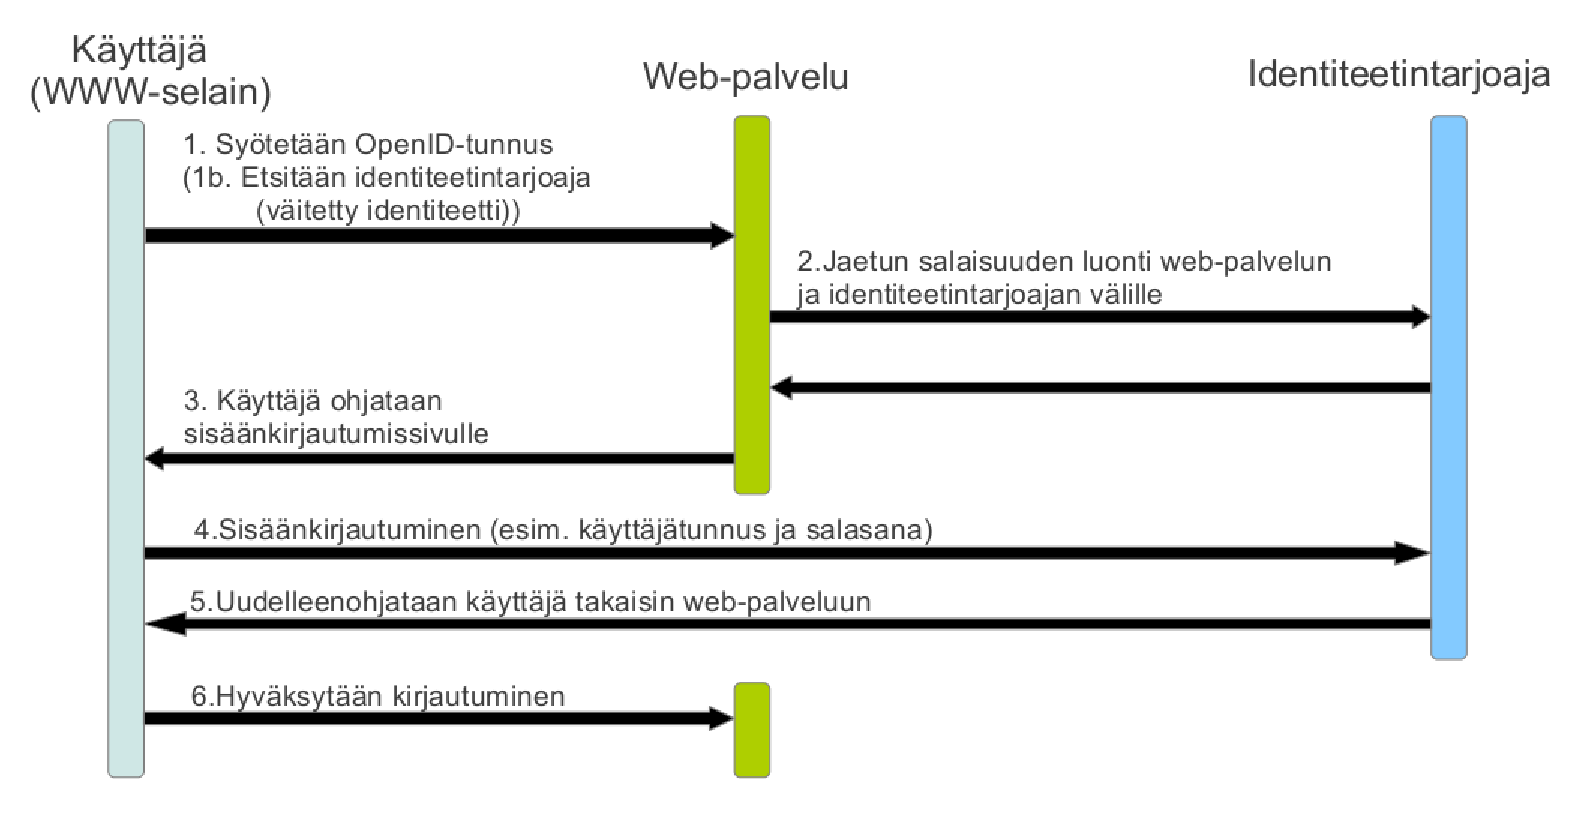
\includegraphics[width=\textwidth]{teknologiat/protokollat/openid.eps}
\caption{OpenID-kirjautumisen vaiheet \cite{openid}.}%
\label{openid_flow}
\end{figure}

OpenID:n suhteen odotukset olivat alkujaan suuria, mutta myöhemmin into protokollan ympärillä on laantunut. Esimerkiksi Microsoftin vuonna 2008 aloittama OpenID-kokeilu lopetettiin elokuussa 2009, minkä jälkeen Microsoft on siirtynyt käyttämään omaa tunnistautumistoteutusta \cite{openid_microsoft}. OpenID-protokollaan liittyvät turvallisuushuolet ovat kasvaneet viime aikoina, koska se koetaan alttiiksi esimerkiksi erilaisille kalasteluhyökkäyksille \cite{billion_keys}.

Julkisen Internetin puolella yleiset OpenID-kir\-jau\-tu\-mis\-si\-vut on korvattu lähes kokonaan eri palveluntarjoajien omilla kirjautumissivuilla. Käyttäjätutkimusten mukaan käyttäjät eivät tunne OpenID:tä, mutta tuntevat palveluntarjoajan kuten Googlen tai Yahoon \cite{refuse_sso}. Näin ollen käyttäjät eivät koe kirjautuvansa OpenID:llä palveluun, johon kirjaudutaan Googlen tunnuksilla. Myös alkuperäinen ajatus siitä, että kuka tahansa voi toimia identiteetintarjoajana, on osoittautunut toimimattomaksi, koska web-palveluiden ylläpitäjät haluavat luottaa päätepisteisiin, joiden kautta heidän palveluun voi kirjautua \cite{refuse_sso}. Tämän vuoksi rajoitetumpaan käyttöön soveltuvat protokollat, kuten OAuth, ovat kasvattaneet suosiotaan.

Standardiin liittyvien ongelmien ja rajoitusten vuoksi on käynyt selväksi, että Open\-ID:n kehitystyötä täytyy jatkaa. Yksi OpenID:n keskeinen rajoitus on, että se varmistaa vain käyttäjän olevan se joka väittää olevansa, mutta se ei ota kantaa käyttäjän pääsyoikeuksiin. Laajentaakseen protokollaa OpenID-säätiö on julkaisemassa uuden OpenID Connect -määritelmän, joka lisää protokollaan myös pääsynvalvonnan \cite{distributed_web_security}. Sen kehitys on kuitenkin vielä niin varhaisessa määrittelyvaiheessa, että sen käyttö tämän tutkielman puitteissa ei ole mielekästä.
\subsubsection{OAauth}
OAuthin kehitystyö alkoi marraskuussa 2006, kun Twitter-pal\-ve\-luun toteutettiin \mbox{OpenID-tukea}. Pian huomattiin, ettei OpenID sovellu käytettäväksi palvelun API-ra\-ja\-pin\-to\-jen kanssa, vaan tarvittiin erillinen pääsynvalvontaprotokolla \cite{oauth_primer}. Siihen asti Twitter-integraatio oli toteutettu pyytämällä käyttäjää antamaan Twitter-tun\-nuk\-sen\-sa ja -salasanansa, joiden avulla palvelu integroitui käyttäjän Twitter-tiliin. Twitterin kehittämä xAuth ja siitä kehittynyt OAuth-protokolla mahdollistavat resurssien käytön ilman käyttäjätunnuksen ja salasanan luovuttamista kolmannelle osapuolelle \cite{oauth2_0}.

OAuthin ensimmäinen versio (1.0) julkaistiin lokakuussa 2007 ja päivitetty versio (1.0a) kesäkuussa 2009 \cite{oauth2_0}. OAuthin versio 2.0 on myös kehitteillä ja se on tarkoitus julkaista marraskuussa 2012 \cite{oauth2_0}. OAuth on määritelty RFC-dokumentissa numero 5849. OAuthin 2.0-version kehitys on ollut vaikeuksissa lähinnä sen jatkuvasti kasvaneiden ominaisuusvaatimusten takia. OAuth 2.0 on kuitenkin käytössä useissa palveluissa, kuten Facebookissa ja GitHubissa, koska OAuth 1.0a:n ominaisuudet eivät ole riittäneet niille. 2.0 helpottaa mm. API-kutsujen tekemistä, koska valtuutusavainten allekirjoitusta on yksinkertaistettu \cite{oauth2_0}.

OAuth on avoin pääsynvalvontaprotokolla hajautetuille web-sovelluksille. Se mahdollistaa käyttäjien resurssien jakamisen palveluiden välillä ilman käyttäjätunnuksen tai salasanan luovuttamista kolmansille osapuolille. Se perustuu erilaisten valtuutusavainten välittämiseen palveluiden kesken \cite{oauth2_0}. Valtuutusavain on allekirjoitettu identiteetintarjoajalla, johon sekä käyttäjä että palvelun toteuttaja luottaa. Muun muassa Facebook tarjoaa avoimen OAuth-rajapinnan, jota web-sovellusten toteuttajat voivat käyttää pääsynvalvonnassaan.

Kuvassa \ref{oauth} on esitetty, kuinka OAuthia käytetään käyttäjän tunnistamiseen. Tunnistautumispalvelin ja käyttäjähallinta voidaan toteuttaa erillisinä palveluina. Tällöin tunnistautumispalvelun antaa pääsyvaltuuden web-sovellukselle, jonka avulla tiedot haetaan käyttäjähallinnasta (kohdat 10 ja 11). Selkeyden vuoksi tunnistautumispalvelun oletetaan toimivan myös käyttäjätietojen jakelijana.

\begin{figure}[!b]
\centering
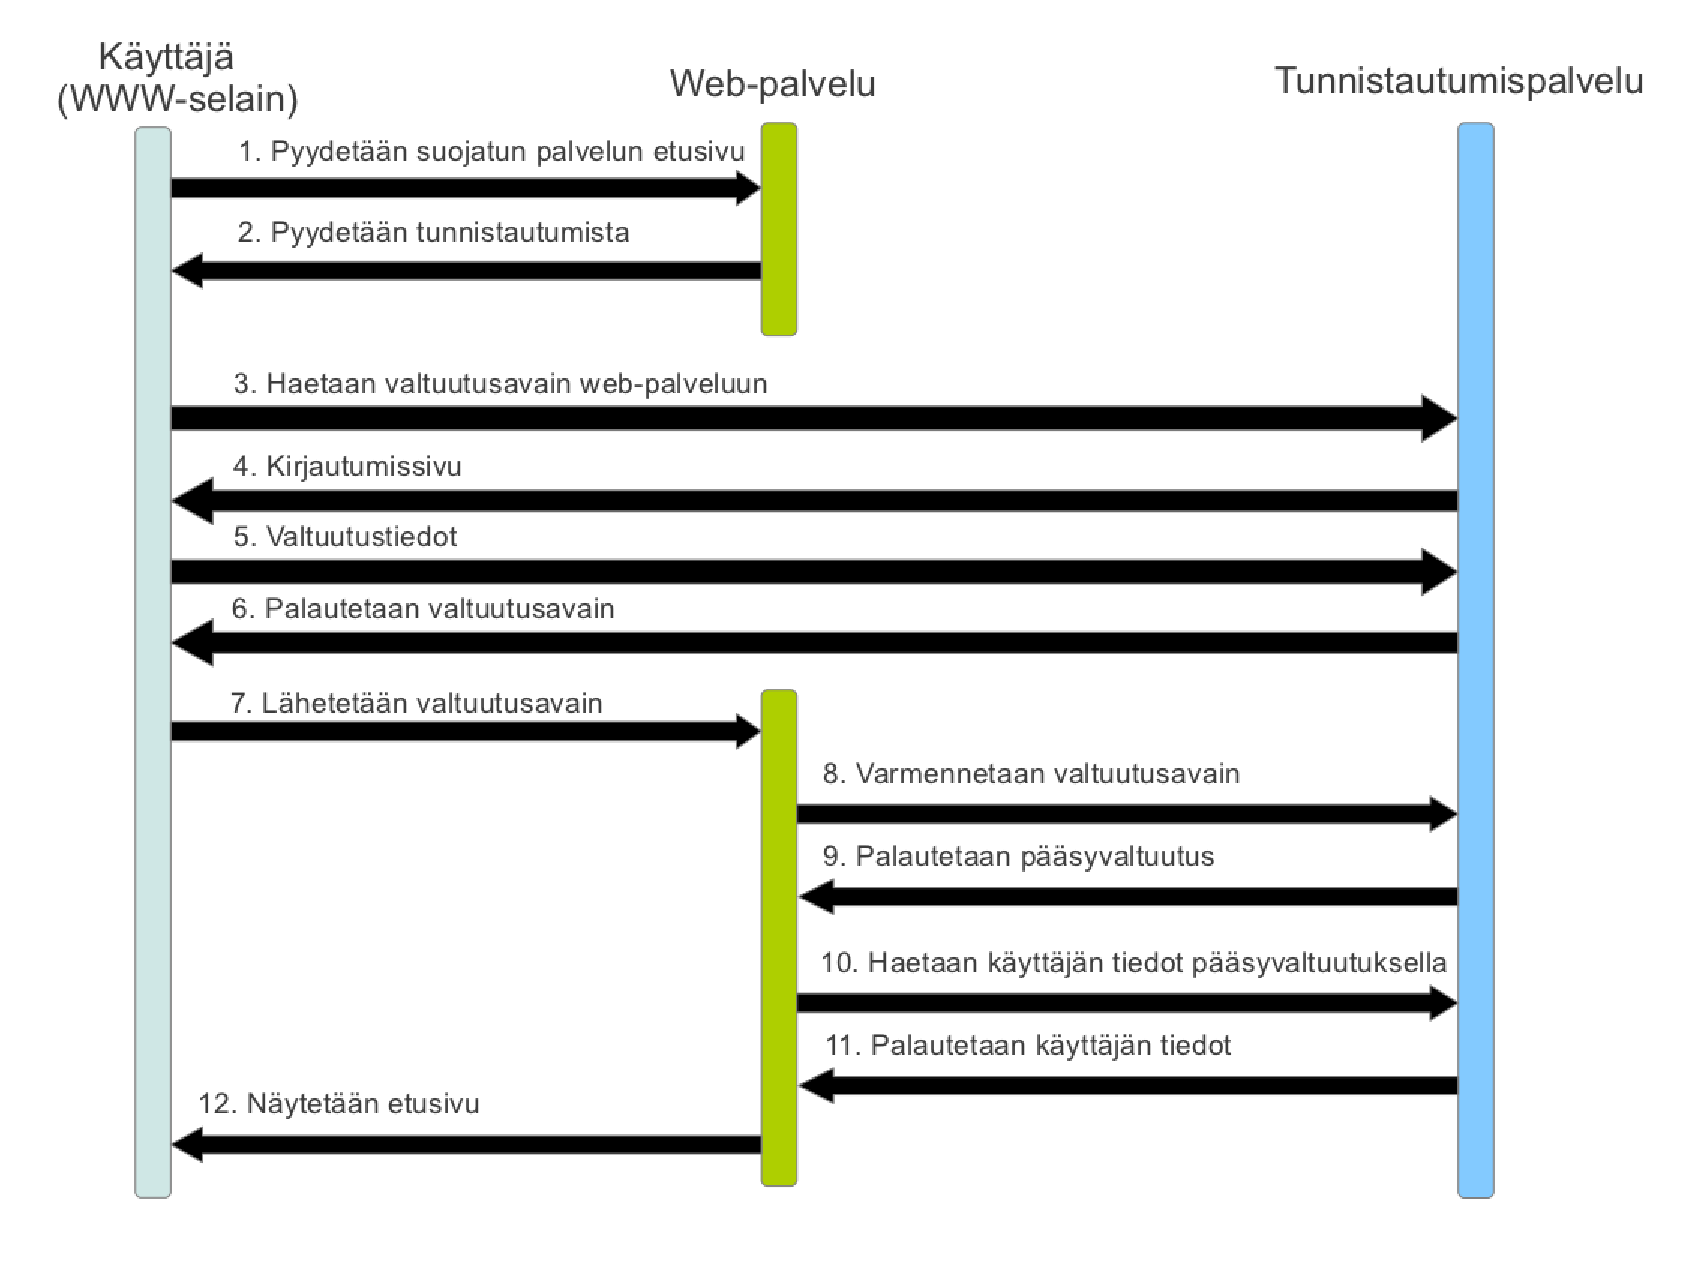
\includegraphics[width=\textwidth]{teknologiat/protokollat/oauth.eps}
\caption{OAuthin toiminta sekvenssikaaviona.}%
\label{oauth}
\end{figure}

OAuthissa valtuutusavaimelle voidaan asettaa erilaisia rajoituksia esimerkiksi sen suhteen, mitä tietoja käyttäjästä annetaan web-sovellukselle tai mihin resursseihin kyseisellä avaimella pääsee käsiksi. Kuvassa \ref{facebook_login} kirjautumisen yhteydessä Porkkanamafialle annetaan oikeus nähdä käyttäjän nimi, profiilikuva, sukupuoli jne. OAuth ei siis ole varsinaisesti tunnistautumisprotokolla, mutta valtuutusavaimen perusteella käyttäjä voidaan yksilöidä: kun käyttäjä kirjautuu myöhemmin uudestaan Porkkanamafiaan, hän hakee valtuutusavaimen Facebookilta, jota käyttämällä Porkkanamafia hakee Facebookista käyttäjän tiedot. Käyttäjän tiedoissa mukana olevalla Facebookin yksilöivällä tunnistenumerolla käyttäjä voidaan todeta samaksi kuin edellisellä kirjautumiskerralla.